\section{Space-Time Cube}\label{sec:space-time-cube}

To fully understand the concept behind the space-time cube, we need to go back to the origin of this visualization.
The original idea for it comes from the 1970s by Torsten Hägerstrand, a Swedish geographer known for his work in time geography.
He introduced the so-called \emph{space-time concept} argued by the fact that time has a critical importance for people fitting
in socio-economic systems. An individual’s life in time-space is defined as a path that starts
when they are born and ends with their death. Because of this, the time component of an individual’s life is of equal
importance as the space component, as they have to pass life’s every point on a timescale~\citep{hagerstrand_1970}.
Hägerstrand used the concept of \emph{space-time path} to show people’s movement through space and time~\citep{corbett2001torsten}.

\begin{figure}[hbt!]
    \begin{center}
        \includegraphics[width=0.4\textwidth]{graphics/2-literature-review/11}
    \end{center}
    \caption{The space-time path~\citep{buard2011visual}}
    \label{fig:figure2.8}
\end{figure}

As mentioned in the previous section, the space-time cube has three dimensions, two represent the spatial component, whereas the
third one represents time. The movement of an object is represented by the trajectory or path during a given time. The cube has
been extensively used for the visualization of trajectories of human activity patterns~\citep{demvsar2010space}. It is also not only a
3D visualization but can be observed as a concept with different operations useful to show static
visualization techniques for temporal data.\footnote{Interesting examples of these operations can be found on the website\\ \url{https://aviz.fr/~bbach/spacetimecubes/}}
One of them is called \emph{time flattening}, as shown in \Cref{fig:figure2.9},
where the cube is flattened along its time axis into a 2D map~\citep{bach2014review}.

\begin{figure}[hbt!]
    \begin{center}
        \includegraphics[width=0.6\textwidth]{graphics/2-literature-review/10}
    \end{center}
    \caption{Time flattening operation}
    \label{fig:figure2.9}
\end{figure}

We saw examples of time flattening in \Cref{fig:figure2.2} and \Cref{fig:figure2.3}. These operations allow the
concept of the space-time cube to be transformed into another form of visualization to extract different details and approaches.
The paper presents the descriptive framework of these operations which are integrated into a variety of fields and gives an insight into them.
We will primarily consider the space-time cube as a 3D visualization with both space and time components, but it is valuable to know that other
types of visualizations can result from it.

One of the most interesting examples of space-time cubes is the 3D visualization of Napoleon’s March mentioned in~\Cref{fig:figure2.2}.
Kraak~\citep{kraak2003geovisualization} transformed the original visualization of the trajectory of the
troops into the space-time cube below. The x- and y-axis represent the spatial attribute of the visualization,
while the z-axis represents time.

\begin{figure}[hbt!]
    \begin{center}
        \includegraphics[width=\textwidth]{graphics/2-literature-review/8}
    \end{center}
    \caption{Napoleon's March space-time cube visualization}
    \label{fig:figure2.10}
\end{figure}

Kraak and Kveladze~\citep{kraak2017narrative} also revisited the
historical event from Napoleon’s March, the crossing of the Berezina River, and introduced the time component to their
2D map (a) to obtain a space-time cube (b). Both Russian (green) and French (blue) troops’ paths were added to the map, and we
can see how multiple space-time paths were integrated into a single cube. They chose this visualization over the traditional
maps because it is more engaging and visually attractive, presenting the narrative of location, attribute, and time perspective.

\begin{figure}[hbt!]
    \begin{center}
        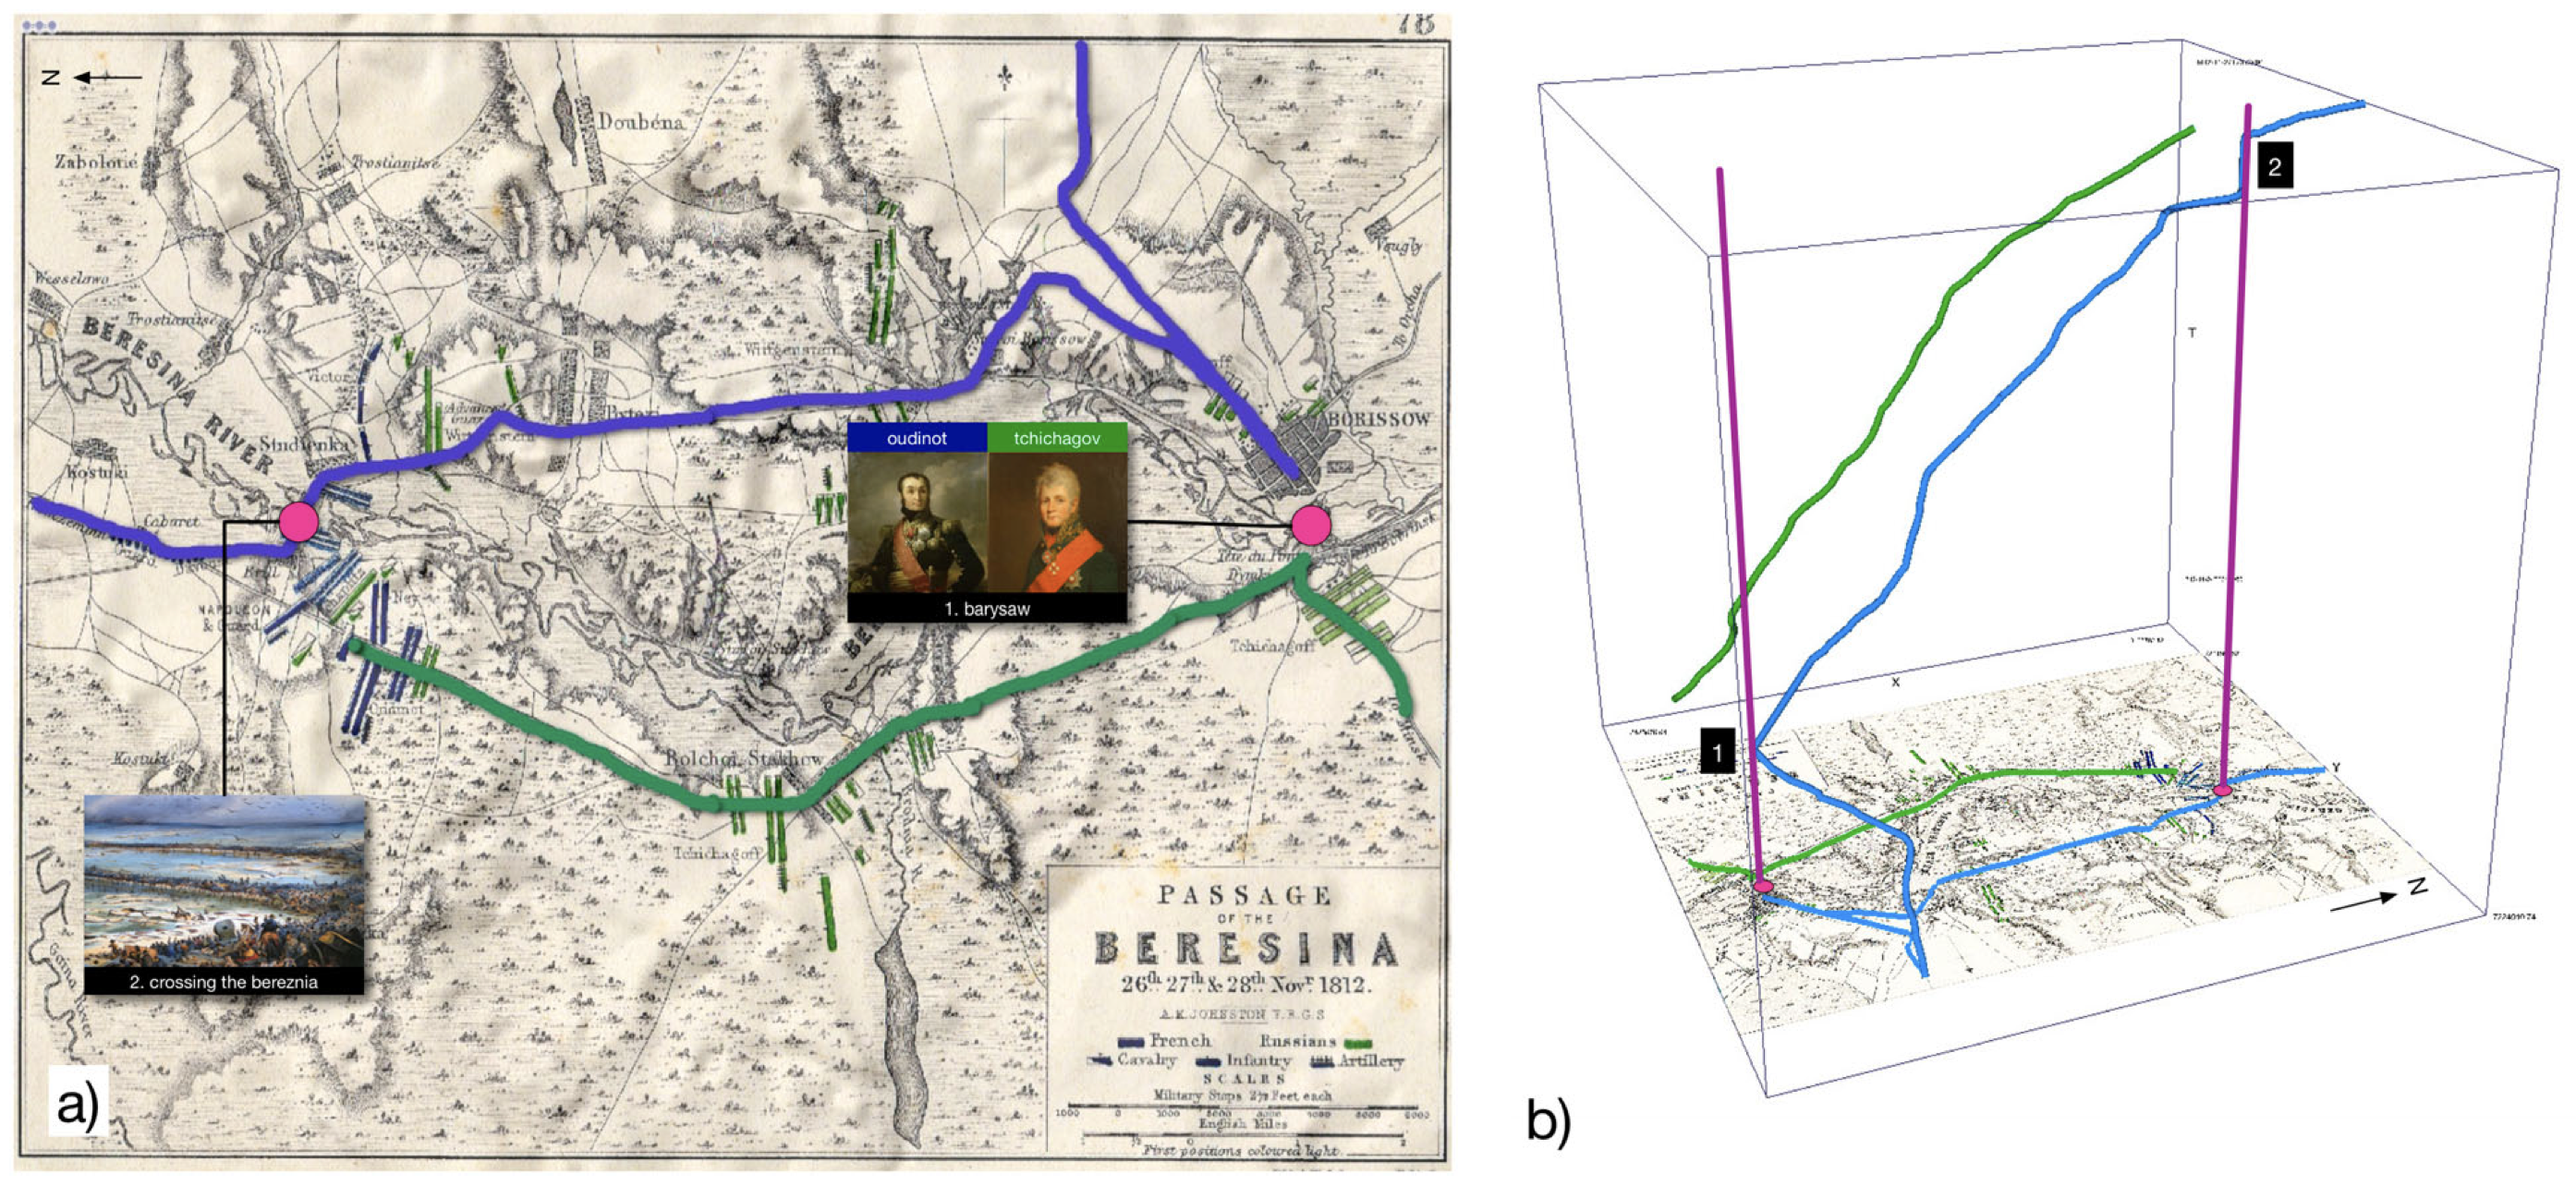
\includegraphics[width=\textwidth]{graphics/2-literature-review/9}
    \end{center}
    \caption{Crossing of Berezina River}
    \label{fig:figure2.11}
\end{figure}

Static 2D maps can show the trajectories of a few objects, but they can
not evaluate elements like speed or if multiple objects met at a crossing in time~\citep{nollenburg2007geographic}.
A space-time cube avoids the above-mentioned trajectory problems because it shows when and not only if an object
visited a place at a given time~\citep{maceachren2005moving}.

Space-time cubes become even more interesting when they are interactive. One example of an interactive cube is Gatalsky et al.~\citep{gatalsky2004interactive}.
They used the cube to represent the earthquakes that happened in the Marmara region, Turkey, from 1976 until 1999. The color or
size of the circles shows different characteristics of events such as the magnitudes of the earthquakes. The dataset contained
10,550 events during that time and representing all of them in the cube resulted in the overlapping and covering of the whole map,
therefore no available patterns for data exploration could be observed. To overcome the problem, they used the temporal focusing
control shown on right in \Cref{fig:figure2.12} and the time interval chosen in the example was 4 months. This approach was
useful for finding clusters in certain areas that might be interesting for seismologists.

\begin{figure}[hbt!]
    \centering
    \begin{subfigure}{.5\textwidth}
        \centering
        \includegraphics[width=0.8\linewidth]{graphics/2-literature-review/12a}
    \end{subfigure}%
    \begin{subfigure}{.5\textwidth}
        \centering
        \includegraphics[width=0.65\linewidth]{graphics/2-literature-review/12b}
    \end{subfigure}
    \caption{The space-time cube of earthquakes in Marmara region, Turkey (left) and the application of temporal focusing to it (right)}
    \label{fig:figure2.12}
\end{figure}

Another more advanced interactive example is the interface for cultural heritage collections by Kraak~\citep{kraak2005timelines} shown
in the figure below.

\begin{figure}[hbt!]
    \begin{center}
        \includegraphics[width=0.85\textwidth]{graphics/2-literature-review/13}
    \end{center}
    \caption{Interactive space-time cube for cultural heritage collections}
    \label{fig:figure2.13}
\end{figure}

The paper states that besides the Time (\emph{when}) and Space (\emph{where}) dimensions, the dimension of Theme (\emph{what}) is of
equivalent value to the selection process of the cultural heritage collection. The space dimension is represented as the map at the
bottom, and the time dimension by the height of the cube with the slider on the left that shows the selected highlighted period
and can be modified by the user. The \emph{what} component is shown inside the cube, with paintings represented by grey
rectangles, and those which satisfy the chosen period condition are shown as artworks' miniatures connected by a line to their location on the
map. This version of the space-time cube has been improved with a timeline as the primary interaction tool, time zooming or focusing,
and joined maps with related symbols~\citep{amini2014impact}.

There are many other space-time cube visualization examples that were not covered here such as~\citep{kraak2003space, kapler2005geotime,
    andrienko2011identifying, nakaya2010visualising, yusof2016interactive, purwanto2021spatiotemporal, mo2020analysis, sen2022characterisation,
    fang2011constructing, wagner2019evaluating, starek2013space},
but it would be impractical to present all of them in this section.

As with every other data visualization, the space-time cube has its advantages and limits depending on the type of data we are trying to
visualize or the subject field related to it. It is important to capture as many of them as possible so that we can improve the final outcome
during the implementation part. Below are some concerns related to the space-time cubes and examples of evaluations done with them.

We have seen multiple examples of the application of a space-time cube in which the context of the data was presented in different ways.
Some used lines as paths to show the movement of an object through space and time, while others used alternative forms (circles, cubes,
etc.) We also saw that it is possible to integrate multiple paths in a single cube, and indeed this visualization is most suitable for 
the display and analysis of paths of different individuals or other objects moving through space~\citep{kraak2003space, persson2020survey}. This
attribute benefits us in the exploration of relationships among multiple artists. On the contrary, with a greater increase in the number of
objects whose movement should be shown in a space-time cube, issues like cluttering or overprinting arise. This prevents reliable visual
identification of patterns inside the cube and the solution to the problem would be to connect the cube to other data visualization
methods~\citep{demvsar2010space}. The most suitable scenario would be to select or filter a group of artists who may be related in a way, not
necessarily as a family, but regarding the \emph{art} part of their lives, and show it in a single cube. This would help experts researching
artists gain more insight into relationships between them. If they belong to an artistic movement (e.g.\ Impressionism) from one historical period
of art, it would be useful to explore their lives and relationships using a visual tool, rather than a written form, and perhaps detect diverse
patterns.

When it comes to the evaluation of the space-time cube, a paper by Kristensson et al.~\citep{kristensson2008evaluation} is known as the first
evaluation of the cube of spatio-temporal data. Participants were exposed to either the space-time cube or another 2D system and asked 15
questions grouped into four categories. The results showed that the cube derived a higher error rate than the 2D representation when simple
questions were asked, but on the other hand, the response time was much lower for the space-time cube when observing complex spatio-temporal
patterns. This suggests that 3D visualization is better when dealing with more complex data patterns.

In another evaluation, Kveladze et al.~\citep{kveladze2012we} discuss the usability of the cube
based on a user-centered design approach. The paper states that the previous evaluations of the cube were mainly the comparison with
other visualization techniques, but they are interested in the cartographic design and its effect on the usability of the cube.
This evaluation was focused on a real case defined by urban geographers and tried to detect an expert's strategy. The goal was to obtain
recommendations and suggestions from the point of view of cartographic design. The experts involved did not have much prior experience with the
space-time cube, so this allowed them to look at the data from a different viewpoint. They recommended the conversion of the
quantitative data scale into a qualitative one. The reason behind this was to profit from the color strength as a visual variable. Also, as
seen previously, data complexity put a constraint on the variables’ usability. The paper also mentions some previous evaluations done on the
space-time cube~\citep{kjellin2008evaluating, willems2011evaluation, kjellin2010different, vrotsou20102d}.
